% This is LLNCS.DOC the documentation file of
% the LaTeX2e class from Springer-Verlag
% for Lecture Notes in Computer Science, version 2.4
\documentclass{llncs}
\usepackage{llncsdoc}
\usepackage[hyphens]{url}
\usepackage[pdftex]{graphicx}     
\usepackage{float}
\usepackage{tablefootnote}
\usepackage{hyperref}

\hyphenation{block-chain}

	%%%%%%%%%%%%%%%%%%%%%%%55
	%% Added to enable numbering for subsubsections, otherwise they would look like paragraphs which is ugly
	%%%%%%%%%%%%%%%%%%%%%%%55
	
	\makeatletter
	\renewcommand\subsubsection{\@startsection{subsubsection}{3}{\z@}%
		{-18\p@ \@plus -4\p@ \@minus -4\p@}%
		{0.5em \@plus 0.22em \@minus 0.1em}%
		{\normalfont\normalsize\bfseries\boldmath}}
	\makeatother
	\setcounter{secnumdepth}{3}

%
\begin{document}


	{
	%
	\title{title\\ - \\ \small Research Paper - Version 0.0\\\small \today}
	
	\author{Benjamin Leiding \and William V. Vorobev}
	
	\institute{ 
		%Chorus Mobility a  Proof-of-Stake Inc. Project\\
		Chorus Mobility\\
		Email: hello@chorus.mobi\\
		%Website: chorus.technology	
	}
	
	\maketitle

	%% ----------------------------------------------------------------
	%% ----------------------------------------------------------------

	\begin{abstract}

		% A good abstract:
		%1.) What is the paper about?
		%2.) What is the SoA?
		%3.) What is the detected gap?
		%4.) What are the main questions to be answered pertaining to the gap?
		%5.) Why is the solution good/better than other solutions?

%		The next generation of tightly interconnected vehicles offers a variety of new technological as well as  business opportunities. Vehicles form so called vehicular ad-hoc networks (VANETs) in order to enable vehicle-to-vehicle (V2V), vehicle-to-infrastructure (V2I), vehicle-to-human (V2H), or in general vehicle-to-everything (V2X) communication and interaction. A variety of manufacturers started implementing specific use cases that are limited to their own products. However, a default interaction standard for this new economy is still missing. Chorus Mobility presents a blockchain-based system that enables a manufacturer agnostic platform solution that allows VANET participants to enact and transact any kind of services and goods. This whitepaper fills the gap in the state of the art by introducing a blockchain-based transaction and interaction layer that enables our V2X platform for goods and services required to kick-start the upcoming V2X economy. We present the advantages of the system, outline the requirements and goals, as well as the architecture of the Chorus V2X platform and eco-system. In addition, we present a prototype that demonstrates how our system helps mitigating traffic congestions and at the same time provides a mean to car insurance companies to incentivize their customers to practice good driving behavior.
 


	\end{abstract}
	
	
	\keywords{keword 1}

	%% ----------------------------------------------------------------
	%% ----------------------------------------------------------------
	
	\section{Introduction}
		\label{s:introduction}

%		Despite steadily growing public transport networks and systems, especially in most first world countries, cars are still the default standard for urban transportation. In the US, ``about 86 percent of all workers commuted to work by private vehicle, either driving alone or carpooling" \cite{mckenzie2015drives}, even though in recent years the numbers remained relatively stable after decades of consistent increase. Similar applies to other industrial countries \cite{netherlandsPublicTransport}\cite{zealand2006car} though the overall percentage of vehicle commuters in Europe is lower than in the US \cite{commuteUSvsEurope}. While it was normal for the last few decades to own a vehicle and commute on a day-by-day basis, the future will be radically different due to the progressing evolution of self-driving cars and autonomous vehicles. The car-sharing economy that developed in recent years in combination with autonomous cars results in a so called \textit{passenger economy} \cite{intelPassengerEconomy}. Users no longer own cars, instead just hop on an autonomous car, pick a destination and get delivered without any human interaction. An Intel report estimates the size of this economy to be around US\$ seven trillion in 2050 \cite{intelPassengerEconomy}.
%		
%		Despite some recent setback, e.g., Uber and Tesla accidents \cite{teslaAccident}\cite{uberAccident}, academic researchers as well as companies from the private sector make fast progress in the research area of self-driving cars. It took less than 15 years from the first DARPA Grand Challenge (a prize competition for autonomous vehicles) to self-driving cars operating on public streets on a regular base (Tesla, Waymo, Uber, etc.) \cite{carStatistics}\cite{carsCalifornia}. Besides these car manufacturers, several projects are also already working on system solutions for trucks, rovers, drones, ships and even airplanes \cite{davWhitepaper}\cite{levander2017autonomous}\cite{trosterer2017transport}. But the progressing automation and driverless transport that enables the passenger economy represents only a small aspect of the potential of these new technologies. During a talk at the 2013 Turing Festival in Edinburgh\footnote{\url{https://www.youtube.com/watch?v=MVyv4t0OKe4}}, Mike Hearn did not only describe a vision where most users do not own cars anymore and instead use services provided by autonomous vehicles that own itself, but also the potentials of a vehicle-to-vehicle (V2V) as well as a vehicle-to-infrastructure (V2I) economy. Autonomous vehicles (AVs) may own themselves, offer services and goods to earn money, and pay money to acquire services that they cannot provide on their own, e.g., cars renting a parking lot, paying for a charged battery, using toll roads, or simple service check ups. The idea of V2V and V2I or in general V2X (vehicle-to-everything) will fuel various new business fields. 
%		
%		Certainly, traditional payment systems such as paper money or fiat currencies in general are not suited to be part of this new economy. There are slow, depend on third parties, e.g., banks, and suffer from bureaucratic overhead. Blockchain technology and cryptocurrencies offer a promising alternative payment solution that comes with several additional technological advantages that we will discuss later on. The blockchain technology, also referred to as distributed ledger system, is most noticeably known for providing the foundation of the peer-to-peer (P2P) cryptocurrency and payment system Bitcoin \cite{nakamoto_bitcoin:2008}, but nowadays there a various different platforms out there, e.g., \cite{tezosWhitepaper}\cite{iotaWhitepaper}\cite{wood2014ethereum}. Several companies already started to prototype applications that combine vehicles and blockchains. Porsche is researching different payment-related applications for vehicles \cite{porscheBlockchain} whereas Ford focuses on traffic marshaling \cite{macneille2018vehicle}. As expected in the early days of a new technology, companies focus on selective solutions for a selection of very specific problems or use cases and the resulting solutions are only compatible with their own products. What is currently missing in the new business field of V2X economy is an industry standard that can easily be integrated with self-driving and (semi)-autonomous cars or even nowadays cars. 

%%%%%%%%%%%%%%%%%%%%%%%%%%%%%%%%%%%%%%%%%%%%%%%%%%%%%%%%%%%%%%%%%%%%%%

%		RQ: How to implement a blockchain-based transaction layer library for (semi)-autonomous vehicles that enables a V2X platform for goods and services?
%		RQ-1: What is the long term vision of Chorus Mobility?
%		RQ-2: What are the critical requirements and the corresponding architecture of the Chorus platform?
%		RQ-3: What are the system-engagement processes for the stakeholders?


%%%%%%%%%%%%%%%%%%%%%%%%%%%%%%%%%%%%%%%%%%%%%%%%%%%%%%%%%%%%%%%%%%%%%%

		This whitepaper addresses the detected gap by introducing the Chorus Mobility solution, thereby answering the question of how to implement a blockchain-based transaction layer that enables a V2X platform for goods and services? In order to answer this question with a separation of concerns, we pose the following sub-questions: What is the long term vision of Chorus Mobility? What are the critical requirements and the corresponding architecture of the Chorus V2X platform? What are the system-engagement processes for the stakeholders?

		The remainder of this paper is structured as follows: Section~\ref{s:section-2} introduces supplementary literature and related work. Section~\ref{s:section-3} outlines the vision of Chorus Mobility. Afterwards, Section~\ref{s:section-4} analyses the requirements of the system and outlines the resulting system architecture that we derive from the requirements. Afterwards, Section~\ref{s:section-5} expands on the system-engagement processes for the stakeholders, followed by Section~\ref{s:section-6} that introduces our prototype. Section~\ref{s:section-7} provides an discussion and an analysis of related projects. Finally, Section~\ref{s:section-8} concludes this work and provides an outlook on future work.


	%% ----------------------------------------------------------------
	%% ----------------------------------------------------------------

	\section{Technical Background and Supplementary Literature}	
		\label{s:section-2}
		
		The following section provides background information and describes related works regarding previous ideas and concepts that focus on a blockchain-based VANET platforms. First, Section~\ref{ss:blockchain-intro} introduces the general concepts of blockchain technology, terms and frameworks. Afterwards, Section~\ref{ss:autonomous-vehicles} and Section~\ref{ss:vanets} focus on the fundamentals of autonomous vehicles as well as vehicular ad-hoc networks. %Finally, Section~\ref{ss:traffic-wave-theory} introduces traffic waves, flows and congestions. 
					
		%% ----------------------------------------------------------------
		%% ----------------------------------------------------------------	
		
		\subsection{Blockchain Technology}
			\label{ss:blockchain-intro}
			
			As the name suggests, a blockchain consists of a chronologically ordered chain of blocks. Every block consists of a certain number of validated transactions and each of those block links to its predecessor by a hash reference. As a result, changing the content of one block also changes all succeeding blocks and hence breaks the chain. All blocks are stored on and verified by all participating nodes. While the initial Bitcoin blockchain only supported a very limited set of scripting instructions, the next generation of blockchain platforms, e.g., Ethereum \cite{wood2014ethereum}, Qtum \cite{qtumWhitepaper}, or Tezos \cite{tezosWhitepaper}, provide Turing-complete programming languages on the protocol-layer level in order to enable smart contract capabilities. Smart contracts are ``orchestration- and choreography protocols that facilitate, verify and enact with computing means a negotiated agreement between consenting parties" \cite{qtumWhitepaper}. Hence, the entities participating in the enactment of a smart contract establish binding agreements and deploy applications using such smart contracts in order to provide blockchain-based applications. Those application are as versatile as smart contracts itself and enable services including the finance sector \cite{nguyen2016blockchain}\cite{saltWhitepaper}, academic and business authentication and identity solutions \cite{leidingUnchained}\cite{CivicWhitepaper}\cite{AuthcoinLeiding2016MCIS}\cite{mccorry2015authenticated}\cite{SelfkeyWhitepaper}, reputation systems \cite{SemadaWhitepaper} as well as platforms for Internet-of-Things (IoT) applications \cite{christidis2016blockchains}\cite{ouaddah2017towards}. 	
			
			The blockchain concept is particularly interesting for the V2X economy for three reasons. First, it removes the need for trusted third parties and instead enables trust-less transaction enactment. Second, transactions that were agreed up on cannot be changed later on since the underlying blockchain is tamperproof. Third, no human interaction is required for any kind of transaction between vehicles or machines in general.

		%% ----------------------------------------------------------------
		%% ----------------------------------------------------------------	
		
		\subsection{Autonomous Vehicles}
			\label{ss:autonomous-vehicles}
			
			Throughout the last 15 years research on autonomous and self-driving cars progressed a lot and nowadays such cars already operating on public streets on a regular base, e.g., Tesla, Waymo and Uber. The ultimate goal of most manufacturers and researchers is to develop the first fully self-driving and autonomous vehicle. In order to clarify some definitions, this section provides a short introduction to the most relevant terms and concepts.

			An autonomous car, also referred to as a driverless car or robotic car, is able to navigate and interact with its environment without human input based on information provided by its sensors \cite{gehrig1999dead}\cite{thrun2010toward}. To do so, modern cars are equipped with radar- and laser sensors, lidars, GPS devices, cameras and several further sensing devices. Based on these information, the vehicle interprets the surrounding world and deduces appropriate action strategies such as avoiding obstacles (other vehicles, humans or a house) on the way to the destination \cite{dokic2015european}\cite{zhu2014vehicle}. As the technology developed over time, vehicles were equipped with more and more sensors, resulting in different driving capabilities. The SAE \cite{autonomyLevelsSAE}
			defined six levels of driving autonomy to categorize the varying capabilities and progresses of several approaches:		
			
			\begin{itemize}
				\item \textbf{Level 0 (No automation): }No driving autonomy, the driver has to perform all driving tasks and interactions.
				\item \textbf{Level 1 (Driver assistance): }The vehicle is controlled by the driver, but is supported by some basic driver assistance functionalities.
				\item \textbf{Level 2 (Partial automation): }The vehicle is able to perform some specific tasks (acceleration or steering) without driver input. Nevertheless, the driver must be fully engaged in driving task and monitor all decision of the car and the environment at all time. The user has to be able to intervene at any given moment. 
				\item \textbf{Level 3 (Conditional automation): }The driver is still a necessity, but is not required to monitor the vehicle or the environment at any given moment. But given a notification by the vehicle, the driver has to be able to take back control over the car in case the vehicle encounters a situation that it cannot deal with on its own.
				\item \textbf{Level 4 (High automation): }The vehicle is able to perform all driving tasks without human intervention in most driving scenarios. The driver can take control whenever desired.
				\item \textbf{Level 5 (Full automation): }The vehicle is able to perform all driving tasks without human intervention in all driving scenarios. The driver can take control whenever desired as long as a steering wheel is still part of the vehicle.
			\end{itemize}
			
			The Chorus interaction- and transaction layer supports and enables a varying number of services for vehicles of each automation level, whereas the most sophisticated applications require SAE level 5 and simpler plug-ins may only require SAE level 0.

		%% ----------------------------------------------------------------
		%% ----------------------------------------------------------------	
		
		\subsection{Vehicular Ad-Hoc Networks - VANETs}
			\label{ss:vanets}

			Communication between vehicles, road infrastructure and Internet-based services is a key enabler for the upcoming generation of vehicles. So called vehicular ad-hoc networks provide an abstract concept that models the different components that are required for V2V, V2I, or V2X communication. Figure \ref{fig:vanets} illustrates the main components of VANETs: Vehicles, on-board-units (OBUs), application-units (AUs) and road-side-units (RSUs).\\
			RSUs are placed  along the road side or in dedicated locations such as at crossroads. Typically, RSUs provide short range communication based on IEEE 802.11p radio technology but can also be equipped with other network devices in order to provide communication within the infrastructural network \cite{al2014comprehensive}. OBUs are mounted onto a vehicle and used for data exchange. To do so, short range wireless- or radio communication is used to exchange these information \cite{baldessari2007car}. Closely linked to the OBU is the AU, they might even reside in the same physical unit or as a mobile until that is regularly removed from the vehicle (e.g smartphones). The AU provides an execution environment for applications that utilize the OBU's communication capabilities \cite{al2014comprehensive}\cite{baldessari2007car}.\\	
			\begin{figure}[ht]
				\centering
				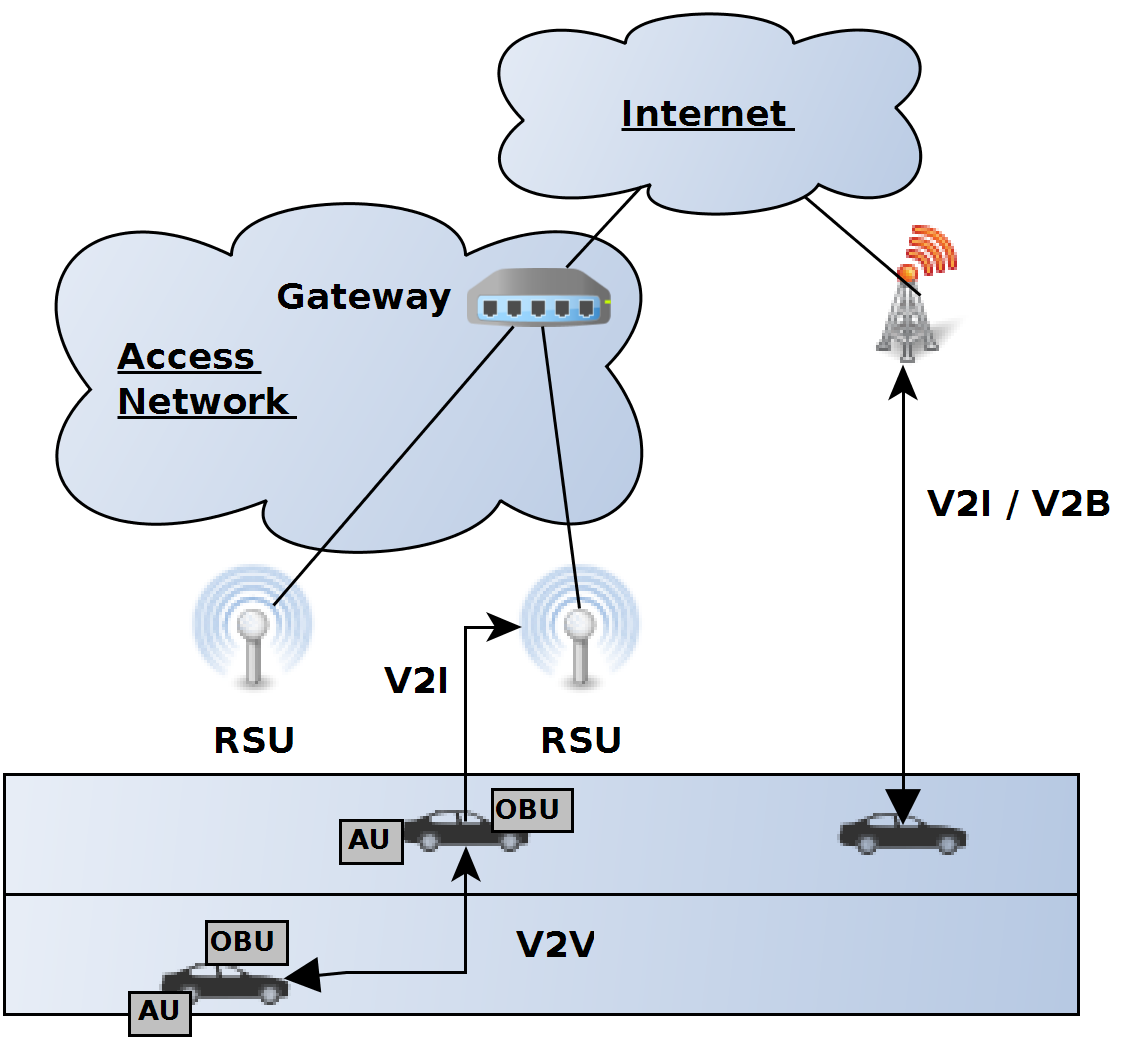
\includegraphics[scale=0.2]{Figures/Vanets.png}
				\caption{General VANET architecture (Based on \protect\cite{baldessari2007car} and \cite{leiding2016self})}
				\label{fig:vanets}
			\end{figure}			
			Communication in VANETs occurs either inside a vehicle between AUs and OBU, wirelessly between different vehicles (V2V), vehicles and infrastructure (V2I) or vehicles and the infrastructure via broadband (V2B) \cite{faezipour2012progress}. For authentication purposes, each network participant is equipped with a unique public/private key pair that resides in a tamper-proof-device (TPD). In blockchain terms, the TPD is similar to an external hardware wallet.
			
		%% ----------------------------------------------------------------
		%% ----------------------------------------------------------------	
		

	%% ----------------------------------------------------------------
	%% ----------------------------------------------------------------

	\section{Section 3}
		\label{s:section-3}
		
	

	%% ----------------------------------------------------------------
	%% ----------------------------------------------------------------
	
	
	\section{Section 3}
		\label{s:section-4}	

	

	%% ----------------------------------------------------------------
	%% ----------------------------------------------------------------
	
	\section{Section 5}
		\label{s:section-5}	
	
	

	%% ----------------------------------------------------------------
	%% ----------------------------------------------------------------

	\section{Section 6}
		\label{s:section-6}	
			
	

	%% ----------------------------------------------------------------
	%% ----------------------------------------------------------------

	\section{Section 7}
		\label{s:section-7}	
		

	
	%% ----------------------------------------------------------------
	%% ----------------------------------------------------------------

	\section{Conclusion and Future Work}
		\label{s:section-8}	

%		This whitepaper presents the Chorus Mobility blockchain-based transaction and interaction layer that enables a V2X platform for goods and services. We outline and describe the technical foundations of this new economy, the longterm vision and benefits as well as the different use cases and scenarios of V2X transactions and interactions, e.g., vehicle-to-vehicle (V2V), vehicle-to-human (V2H), or vehicle-to-infrastructure (V2I).
%		
%		Based on the use cases and scenarios we identify the requirements and criteria that a blockchain-based V2X transaction and interaction layer protocol must satisfy. With respect to functional and non-functional requirements, Chorus aims to develop a blockchain- as well as manufacturer agnostic and interoperable V2X platform that enables interaction and transaction between participating entities and a plug-in interface for external applications.
%		Subsequently, we derive the service-oriented architecture of the system based on the identified requirements and goals. We present the system architecture using technology-agnostic UML-component and sequence diagrams that detail the system’s main components and communication interfaces. In order to ensure widespread adoption, special focus will be given in the future to the API design and library integration for car manufacturers.
%		
%		A core element of many of the Chorus use cases is smart contract-based negotiation and contract enactment between
%		entities that are the result of collaborating tasks and subprocesses. On an abstract level, most of the use cases presented in this paper follow a similar workflow on the smart-contract level. Hence, we decided to integrate an abstract smart contract negotiation lifecycle that we describe. The lifecycle is divided into the different stages (preparatory, negotiation, contract execution, rollback and contract expiry stage) that we explain in detail. Furthermore, we designed two auction algorithms for the V2X economy that allow to reach an efficient consensus on a certain price between buyer and seller. Our auction algorithms are based on the concept of so called Vickrey Auction, and we envisioned one algorithm for one-to-one interaction as well as a second workflow for scenarios with multiple buyers and sellers. Finally, we present the Chorus token value proposition and the surrounding token economy eco-system that fuels the V2X platform.
%		
%		Next, we present a Chorus prototype implementation. We demonstrate how our protocol can help mitigating traffic congestions and at the same time provides a mean to car insurance companies to incentivize their customers to practice good driving behavior. 	
%		
%		Future releases will focus on the longterm vision of Chorus Mobility and the development of the abstract transaction and interaction layer as well as the API and library integration. Besides that, we will also continue to focus on further research aspects of the upcoming V2X economy that will facilitate future developments of Chorus Mobility.

	%% ----------------------------------------------------------------
	%% ----------------------------------------------------------------


	\label{Bibliography}
	\bibliographystyle{splncs03}
	\bibliography{Bibliography}
	
	%% ----------------------------------------------------------------
	%% ----------------------------------------------------------------	



	%
\end{document}


